\chapter{Ein Überblick über Clusteranalyseverfahren}

Eine Clusteranalyse oder auch Klassifizierung dient dazu, Objekte und/oder Merkmale zu klassifizieren. Dabei sollen Merkmale und/oder Objekte in möglichst homogenen Klassen, die untereinander möglichst heterogen sind, zusammengefasst werden.

Nach \citet[S. 476]{Backhaus.2016} lassen sich vier übergeordnete Gruppierungen von Clusteranalyseverfahren darstellen. Abbildung \ref{pic:backhaus476} gibt hierzu nochmal einen Überblick.

\begin{enumerate}
	\item \textit{Partitionierende Verfahren}: Diese Algorithmen benötigen eine vorgegebene Clusteranzahl, in die sie die Objekte einzuordnen versuchen. Unterschiede zwischen den einzelnen Verfahren entstehen hierbei vor allem durch die unterschiedliche Messung der Verbesserung der Clusterbildung und in der Regelung des Austauschs der Objekte zwischen den Clustern, weswegen man diese Clusteranalyseverfahren auch in Austauschverfahren und iterierte Minimaldistanzverfahren unterscheiden kann.
	\item \textit{Hierarchische Verfahren}: Im Gegensatz zu partitionierenden Verfahren benötigen diese Algorithmen keine vorgegebene Clusteranzahl, sondern iterieren alle möglichen Clusteranzahlen durch. Hierarchisch divisive Verfahren gehen dabei von der größtmöglichen Partition aus, die sie Schritt für Schritt in die kleinstmöglichen Partitionen zerlegen (ein Objekt in einer Partition). Hierarchisch agglomerative Verfahren dagegen fassen die feinsten Partitionen zu immer größeren Gruppen zusammen, bis schließlich die größtmögliche Partition erreicht ist, die alle Objekte enthält. Abbildung \ref{pic:xu21} zeigt diesen Unterschied deutlich.
	\begin{figure}[h]
		\begin{center}
			\includegraphics[width=8cm]{pics/xu21.png}
		\end{center}
		\caption{Vergleich der agglomerativen und divisiven Strategien nach \citet[S. 21]{Xu.1999}}
		\label{pic:xu21}
	\end{figure}
	\item \textit{Graphentheoretische Verfahren}
	\item \textit{Optimierungsverfahren}
\end{enumerate}

\newpage % Könnte Probleme verursachen, wenn sich der Text verschiebt!

\begin{figure}[h]
	\begin{center}
		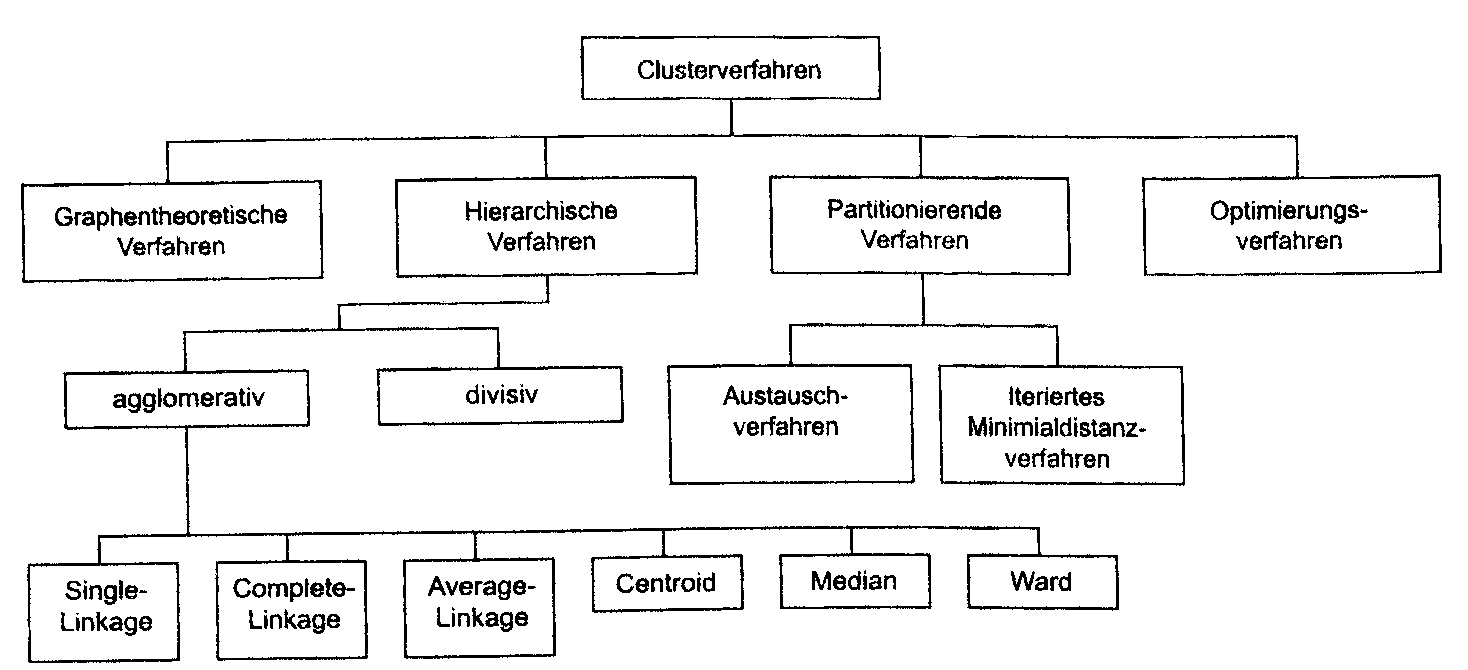
\includegraphics[width=14cm]{pics/backhaus476.png}
	\end{center}
	\caption{Gruppierungen nach \citet[S. 476]{Backhaus.2016}}
	\label{pic:backhaus476}
\end{figure}

\begin{figure}[h]
	\begin{center}
		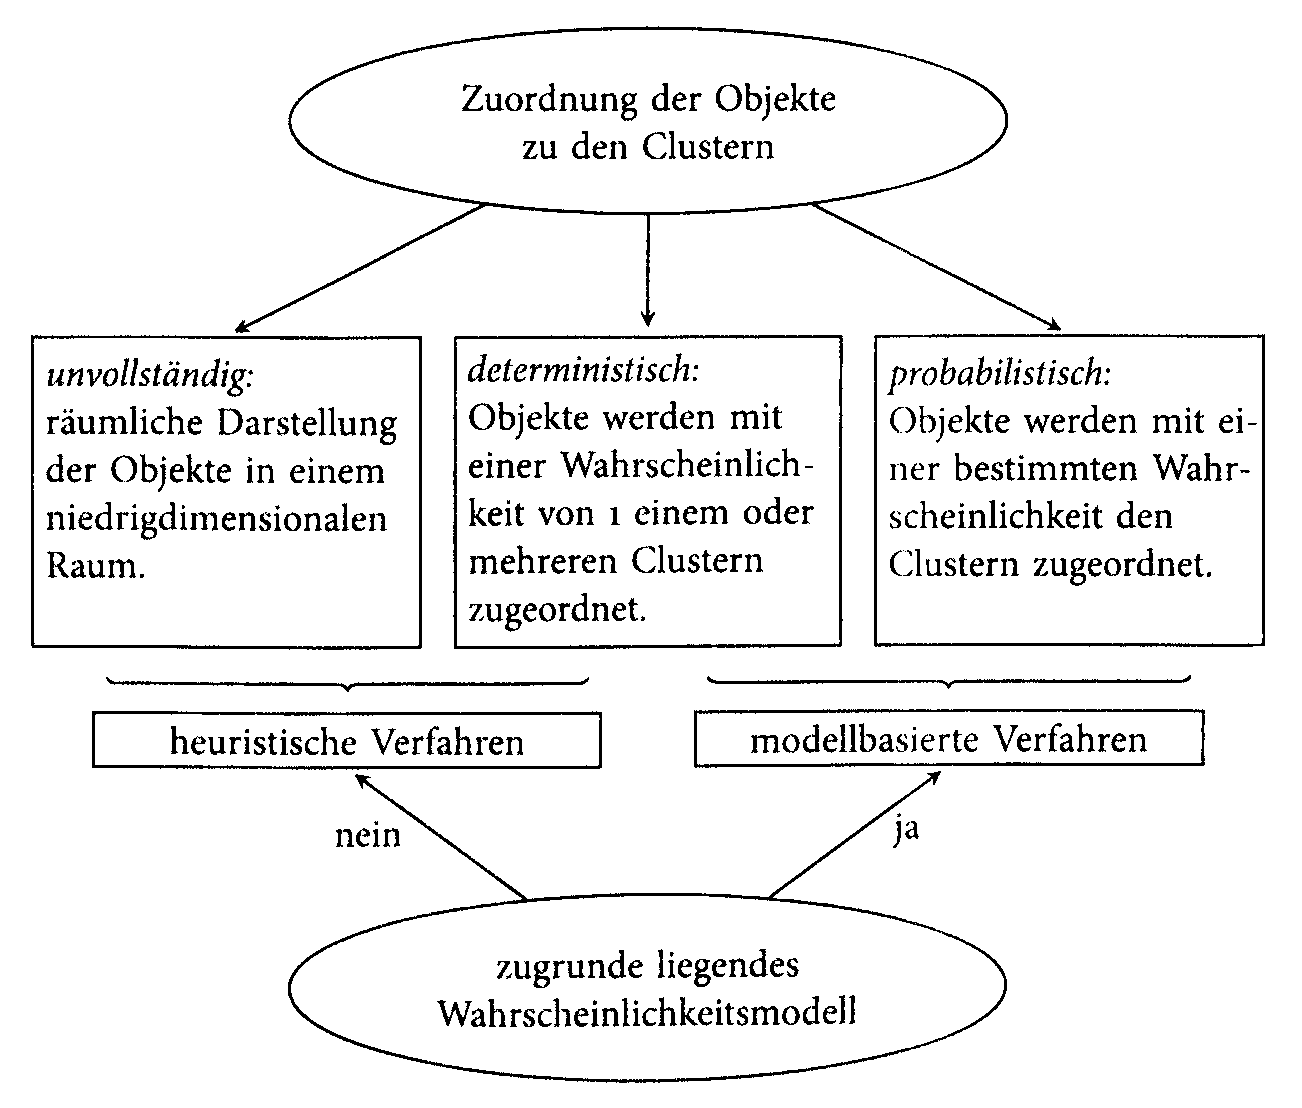
\includegraphics[width=10cm]{pics/bac20.png}
	\end{center}
	\caption{Wahrscheinlichkeitsmodelle nach \citet[S. 20]{Bacher.2010}}
	\label{pic:bac20}
\end{figure}

\citet[S. 18]{Bacher.2010} unterscheiden Clusteranalyseverfahren anders auf Grundlage der Zuordnung der Klassifikationsobjekte zu den Clustern:

\begin{enumerate}
	\item \textit{Unvollständige Clusteranalyseverfahren} (auch \textit{geometrische Methoden}, \textit{Repräsentations-} oder \textit{Projektverfahren}): Diese Verfahren führen nur zu einer räumlichen Darstellung und sind somit für den menschlichen Beobachter nur bis in den dreidimensionalen Raum möglich. Probleme mit mehr als drei Dimensionen können mit ihnen also schwer behandelt werden.
	\item \textit{Deterministische Clusteranalyseverfahren}: Die Klassifikationsobjekte werden mit einer Wahrscheinlichkeit von 0 oder 1 einem Cluster zugeordnet. 
	\item \textit{Probabilistische Clusteranalyseverfahren} (auch \textit{Fuzzy-Clusteranalyse}): Die Klassifikationsobjekte werden verschiedenen Clustern mit einer Wahrscheinlichkeit zwischen 0 und 1 zugeordnet. Diese Verfahren stellen im Grunde eine Verallgemeinerung der Deterministischen Clusteranalyseverfahren dar, da sie die Annahme fallen lassen, dass die Klassifikationsobjekte mit einer Wahrscheinlichkeit von 0 oder 1 zugeordnet werden.
\end{enumerate}

\citet[S. 21]{Bacher.2010} unterscheiden die Verfahren weiterhin auch aufgrund ihres zugrundeliegenden Wahrscheinlichkeitsmodells. Abbildung \ref{pic:bac20} zeigt auf, welcher Zuordnung welches Wahrscheinlichkeitsmodell zugrunde liegt. 